
%\subsection{Decays to two W bosons}

%As depicted in Fig.~\ref{fig:higgsBR}, the branching fraction of the
%Higgs boson to two W bosons is the largest of the branching fractions
%for Higgs mass above 135~\GeV, and enjoys a factor of 2-3 over the
%branching fraction to two Z bosons for most of the presented mass
%range. As with the Z boson, the dominant decay of a W boson is to
%quarks. The fully hadronic decay of the Higgs boson through two W
%bosons is not studied, since it is nearly impossible to distinguish
%from SM backgrounds. Therefore the study of $\PH\to\PW\PW$, contrary
%to $\PH\to\cPZ\cPZ$, always includes at least one neutrino that escapes
%the detector as missing energy.

\subsection{$\PH \to \PW\PW \to \ell\ell\nu\nu$}

In this search channel, the Higgs boson decays to two \PW\ bosons, both
of which decay leptonically, resulting in a signature with two isolated,
oppositely charged, high-$\pt$ leptons (electrons or muons) and large
$\MET$ due to the undetected neutrinos.
The events are selected by triggers that require the presence of one or
two high-$\pt$ electrons or muons. 
%Two 
%oppositely charged lepton candidates are required, 
Two leptons are required to be reconstructed with $\pt
>20\GeV$ for the leading lepton ($\ptlmax$) and $\pt >10\GeV$ for the
trailing lepton ($\ptlmin$).  Only electrons (muons) with $|\eta|
<$2.5 (2.4) are considered in the analysis.

Events are classified according to the number of selected jets
with $\Et>30\GeV$ and $|\eta|<$4.7
%The inclusion of two such leptons in the search strongly suppresses
%QCD multijet and inclusive \PW+jets backgrounds, which have large
%production cross sections at the LHC.
%This channel participated in the discovery of the new
%``SM-Higgs-like'' boson and is described in~\cite{cmsobsboson}.
%Previous searches in this mode can be found
%in~\cite{HWW2010,HWW2011}. 
%Events are separated by jet multiplicity
into three mutually exclusive categories, which are characterized by
different signal yields and signal-to-background ratios.  In the
following we call these the 0-jet, 1-jet and 2-jet samples.  Events
with more than two jets are not considered.  Furthermore, the search
strategy splits signal candidates into same-flavor lepton category 
%lepton ethree final states denoted
(\Pep\Pem, \mumu) and different-flavor lepton category ($\Elpm\Mmp$).
The bulk of the signal arises through direct $\PW$ decays to electrons
or muons, while a 
% of opposite charge, where the 
small contribution proceeding
through an intermediate $\Pgt$-lepton decays is implicitly included.  
The different-flvor lepton 0- and 1-jets categories are
analysed with a multivariate technique (MVA), while all others make use of a
selection criteria based on sequential cuts.
More details about the analysis can be found 
in Refs.~\cite{Chatrchyan:2012ty,cmsobsboson}.

%The events are selected by triggers that require the presence of one or
%two high-$\pt$ electrons or muons. 
%Two oppositely charged lepton candidates are required, with $\pt
%>20\GeV$ for the leading lepton ($\ptlmax$) and $\pt >10\GeV$ for the
%trailing lepton ($\ptlmin$).  Only electrons (muons) with $|\eta|
%<$2.5 (2.4) are considered in the analysis.

%A multivariate selection is applied to separate jets from the primary
%interaction from those reconstructed due to energy deposits associated
%with pile-up. The discrimination is based on the differences in the
%jet shapes, in the relative multiplicity of charged and neutral
%components and in the different fraction of transverse momentum which
%is carried by the hardest components.  Within the tracker acceptance
%the jet tracks are also required to be compatible with the primary
%vertex. Events are classified according to the number of selected jets
%with $\Et>30\GeV$ and $|\eta|<$4.7.

In addition to high-$\pt$ isolated leptons and minimal jet
activity, $\MET$ is present in signal events but
generally not in background. For this channel, a
\textit{projected}~$\MET$ variable is employed. It is equal to the
component of $\MET$ transverse to the nearest lepton if the difference
in azimuth between this lepton and the $\MET$ vector is less than
$\pi/2$. If there is no lepton within $\pi/2$ of the direction of
$\MET$ in azimuth, $\MET$ is used directly.  Since the
\textit{projected}~$\MET$ resolution is degraded by pileup, the
minimum of two $\MET$ observables is used: the first includes all
reconstructed particles in the event, while the second uses only the
charged particles associated with the primary vertex.  Events with
\textit{projected}~$\MET$ above 20$\GeV$ are selected for this
analysis.

The various backgrounds are suppressed using techniques described
in~\cite{cmsobsboson}. Top-quark backgrounds are controlled with a
top-tagging technique based on soft-muon and b-jet
tagging~\cite{CMS-PAS-BTV-11-003}. A minimum dilepton transverse momentum
($\pt^{\ell\ell}$) of 45 $\GeV$ is required to reduce the $\Wjets$
background. Rejection of a third lepton passing the identification and
isolation requirements reduces both $\WZ$ and $\wgamma$ backgrounds,
where in the latter case a photon is misidentified as an electron.The
background from low mass resonances is rejected by requiring a
dilepton mass ($\mll$) greater than 12 $\GeV$.

The Drell-Yan process produces same-flavor lepton pairs ($\Elp\Elm$
and $\Mp\Mm$), therefore a few additional requirements are applied in the
same-flavor final states.  First, the resonant component of the
Drell-Yan production is rejected by requiring a dilepton mass outside
a 30\GeV window centered on the $\Z$ mass.  Then, the remaining
off-peak contribution is suppressed by requiring the minimum of
the two \textit{projected}~$\MET$ variables to be greater than 45
$\GeV$. For events with two jets, the dominant source of fake
\MET\ is the mismeasurement of the hadronic recoil and the optimal
performance is obtained by simply requiring $\MET > 45 \GeV$.
 Finally, the momenta of the dilepton system and of the most energetic
jet must not be back-to-back in the transverse plane. These selections
effectively reduce the Drell-Yan background by three orders of
magnitude, while rejecting less than 50\% of the signal.

These requirements comprise a set of ``preselection'' criteria.
%After applying these criteria, the observed yields in data are in the
%1-1.5 thousand event range for all three jet categories. 
This sample
is dominated by non-resonant $\WW$ events.  
%The main efficiency loss
%is due to the lepton selection and the stringent $\MET$ requirements.
Figure~\ref{fig:hww2l2n_bdt_500}(a) shows the $m_{\ell\ell}$
distribution
for the 0-jet category
after the preselection. 
The data are compared to MC predictions for major backgrounds and
a signal hypothesis for a SM Higgs boson with mH = 500~\GeV.

After preselection, a multivariate technique is employed for the
different-flavor final state in the 0-jet and 1-jet
categories. In this approach a boosted decision tree (BDT) is
trained~\cite{tmva} for each Higgs-boson-mass hypothesis and jet
category to discriminate signal from background. 
To enhance the signal-to-background ratio
%in addition to the pre-selection criteria
loose $\mH$-dependent requirements are
applied 
 on $\mll$ and
the transverse mass
\begin{equation} 
m_\mathrm{T}^{\ell\ell,\MET} = \sqrt{2 \pt^{\ell\ell} \MET (1-\cos\delphimetll)}\ ,
\nonumber
\end{equation}
where
$\delphimetll$
is the difference in azimuth between $\MET$ and $\pt^{\ell\ell}$).

The multivariate technique employs the
variables used in the preselection, and some additional observables like
$\Delta R_{\Lep\Lep}$
between the leptons and the $m_\mathrm{T}^{\ell,\MET}$. 
For the 1-jet category the $\delphimetll$ and
azimuthal angle between the
$\pt^{\ell\ell}$ and the
highest $\pt$ jet are also used. The BDT-classifier distributions for $\mH=500\GeV$
are shown in Fig.~\ref{fig:hww2l2n_bdt_500}(b) for the 0-jet
category.  The BDT training is performed using $\Hww$ as signal and
non-resonant $\WW$ as background. The binned BDT distributions are
fitted to templates for the signal and background BDT distributions.

%Parallel analyses were performed as a cross-check for the BDT, one
%using simpler selection criteria optimized for each mass hypothesis,
%and another using a Matrix Element method as previously done
%in~\cite{Aaltonen:2008ec}, to compute the differential cross section
%for signal and background hypotheses on an event-by-event basis.  All
%approaches yield results consistent with those from the BDT analysis.

The 2-jet category is optimized for the VBF
production mode
\cite{Ciccolini:2007jr, Ciccolini:2007ec, Arnold:2008rz,Cahn:1987}, whose
cross section is roughly ten times smaller than that of the
gluon-gluon fusion mode. Selection criteria based on sequential set
of cuts are employed for
this category. The selections is independent on the Higgs mass
hypothesis, except a loose requirement on the dilepton mass.

\begin{figure}[htbp]
\centering
%   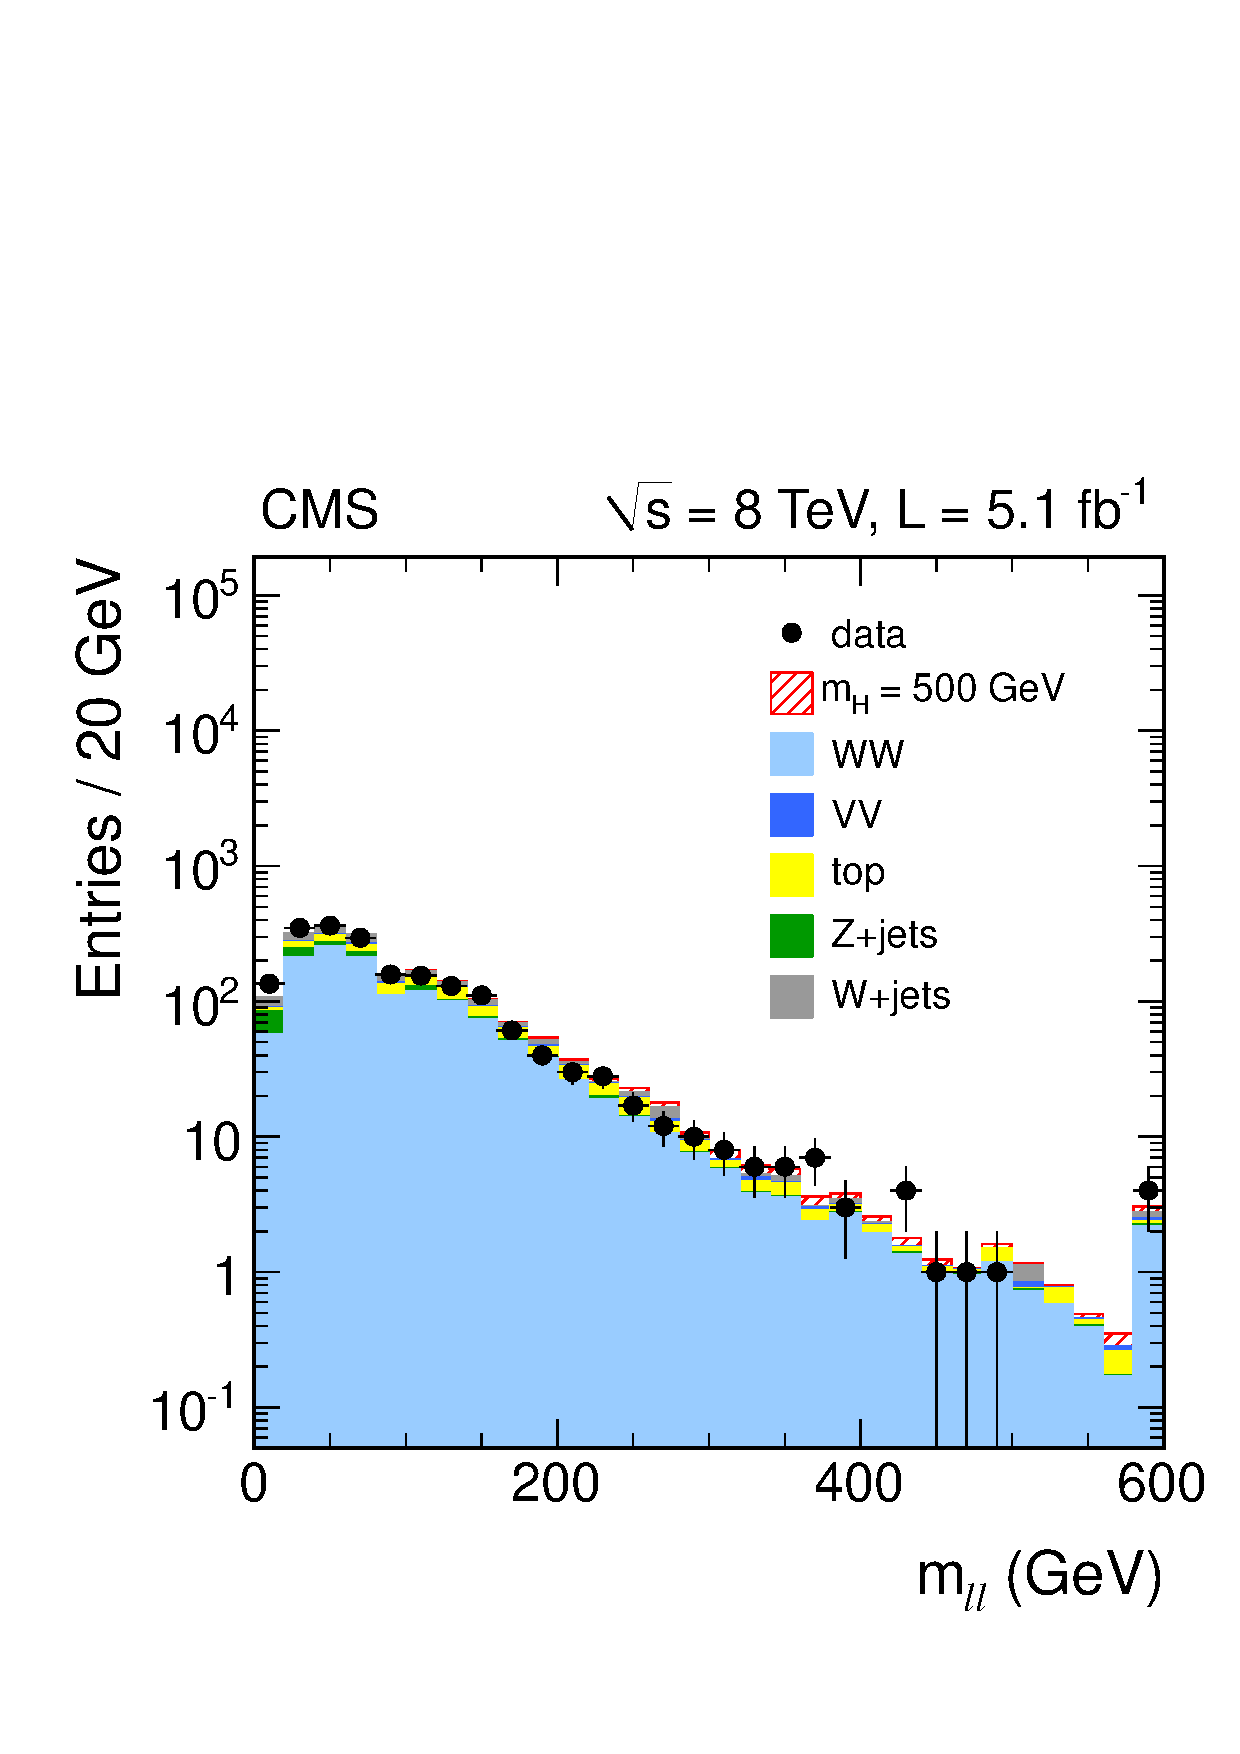
\includegraphics[width=0.49\textwidth]{plots/hww2l2n_highmass_mll500_0j.pdf}
%   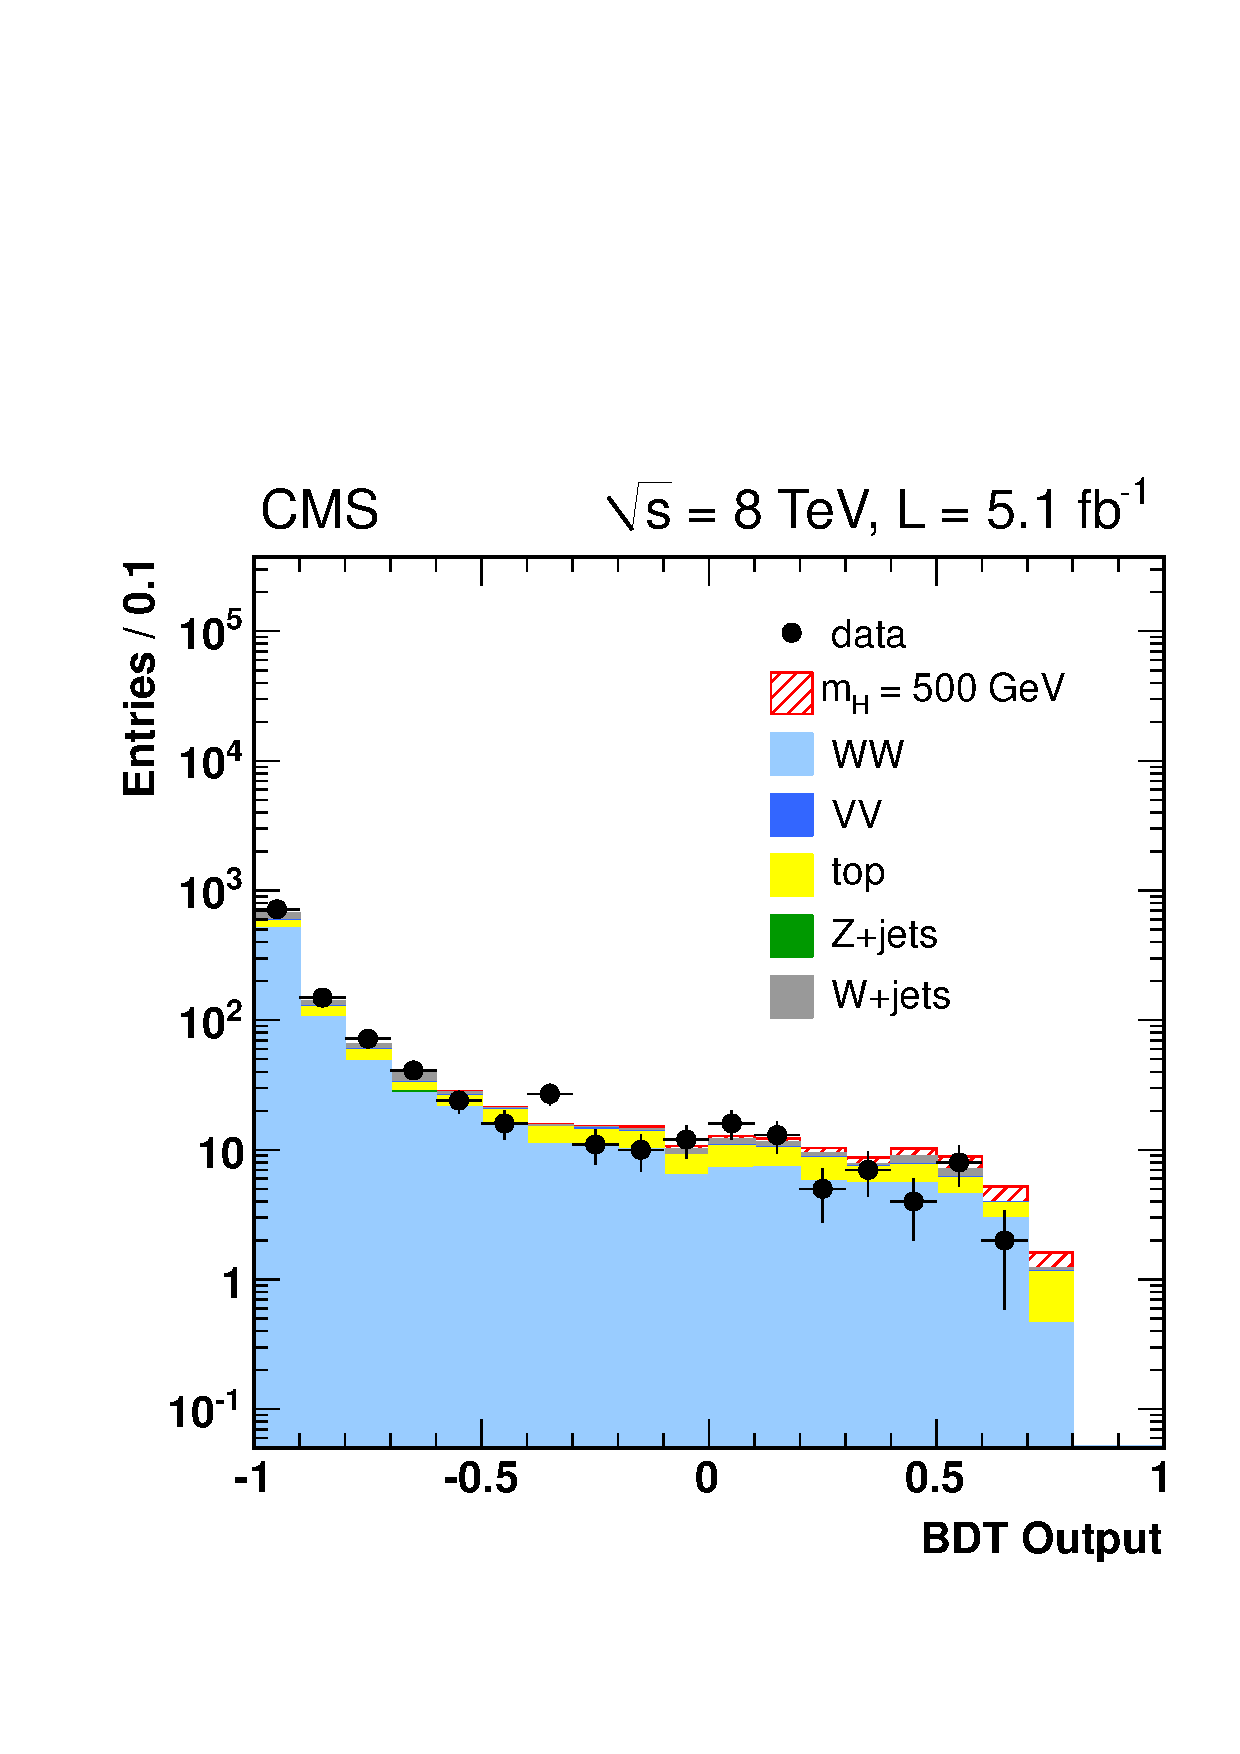
\includegraphics[width=0.49\textwidth]{plots/hww2l2n_highmass_bdt500_0j.pdf}
   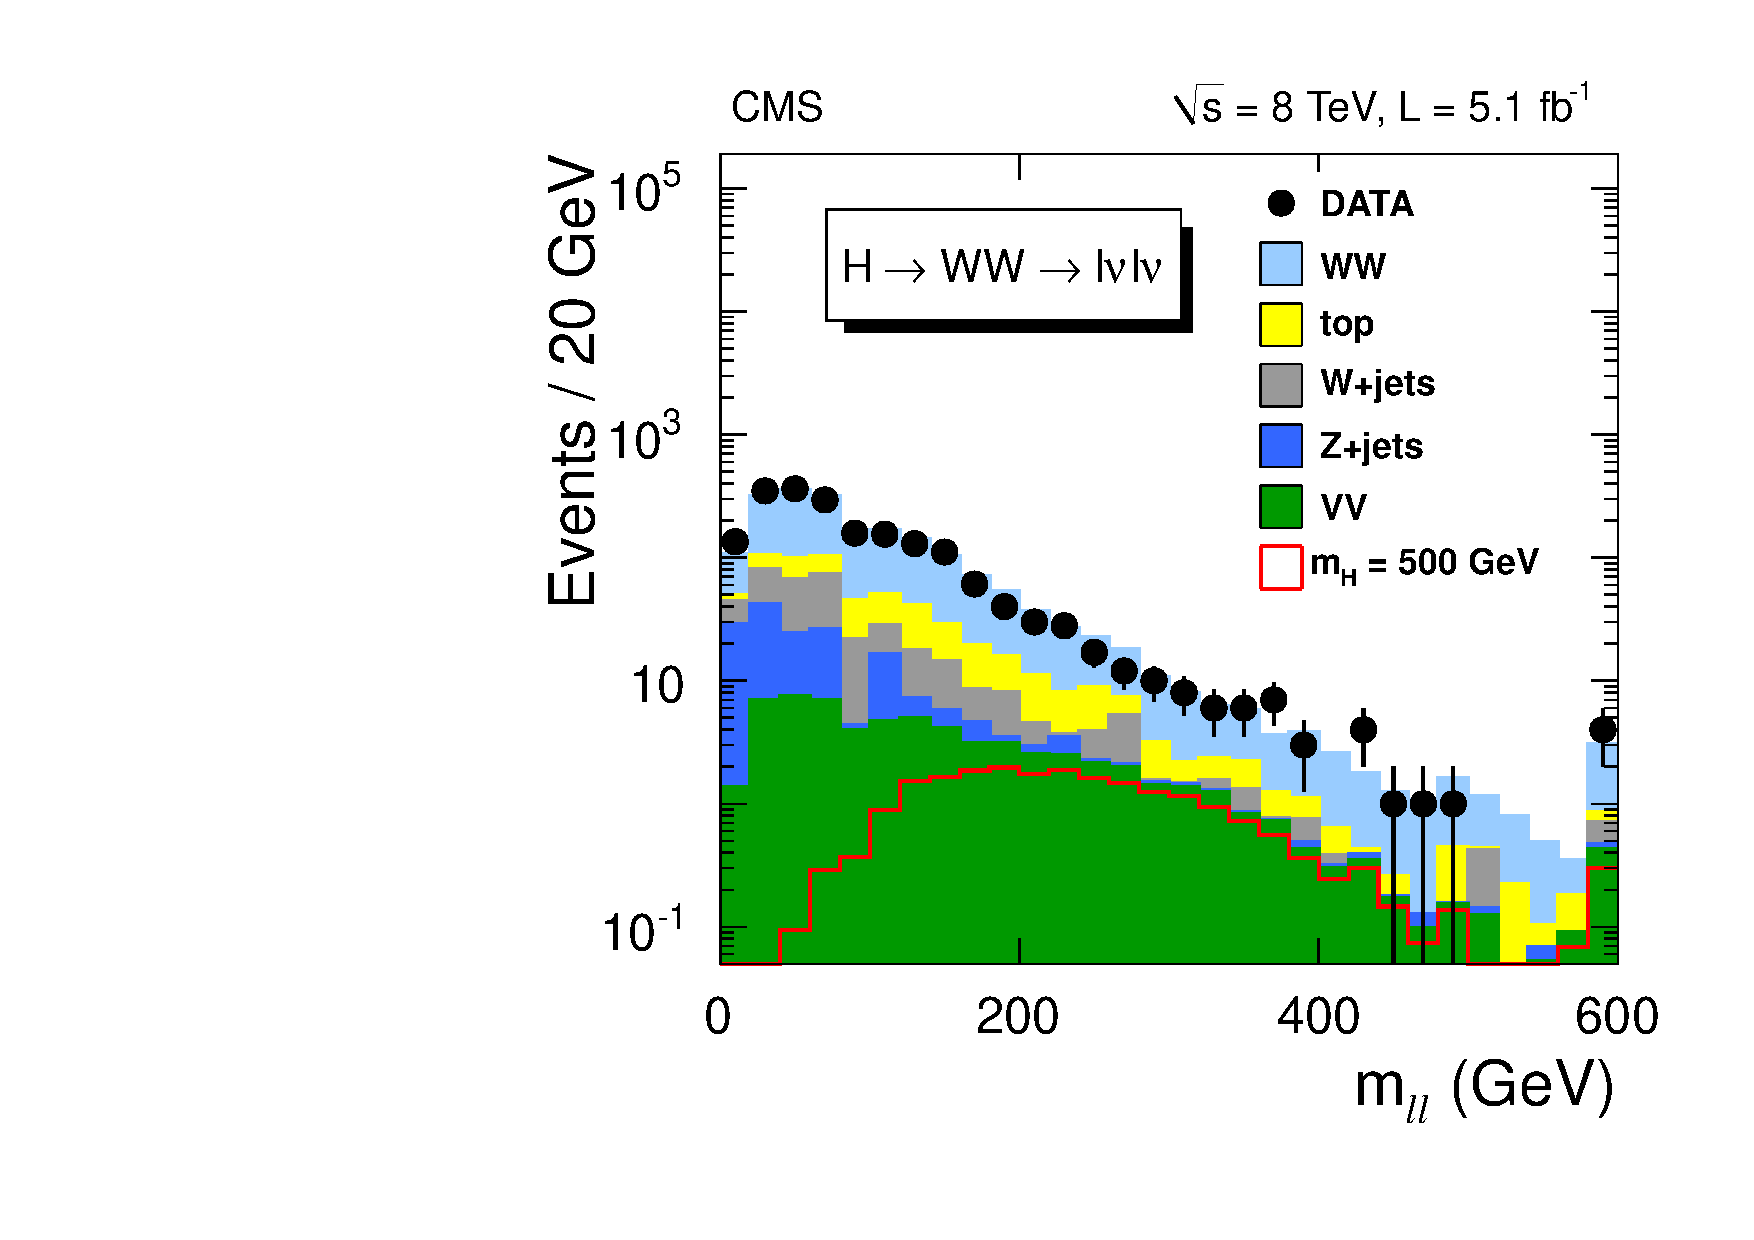
\includegraphics[width=0.49\textwidth]{figures/WW2l2nuMass.pdf}
   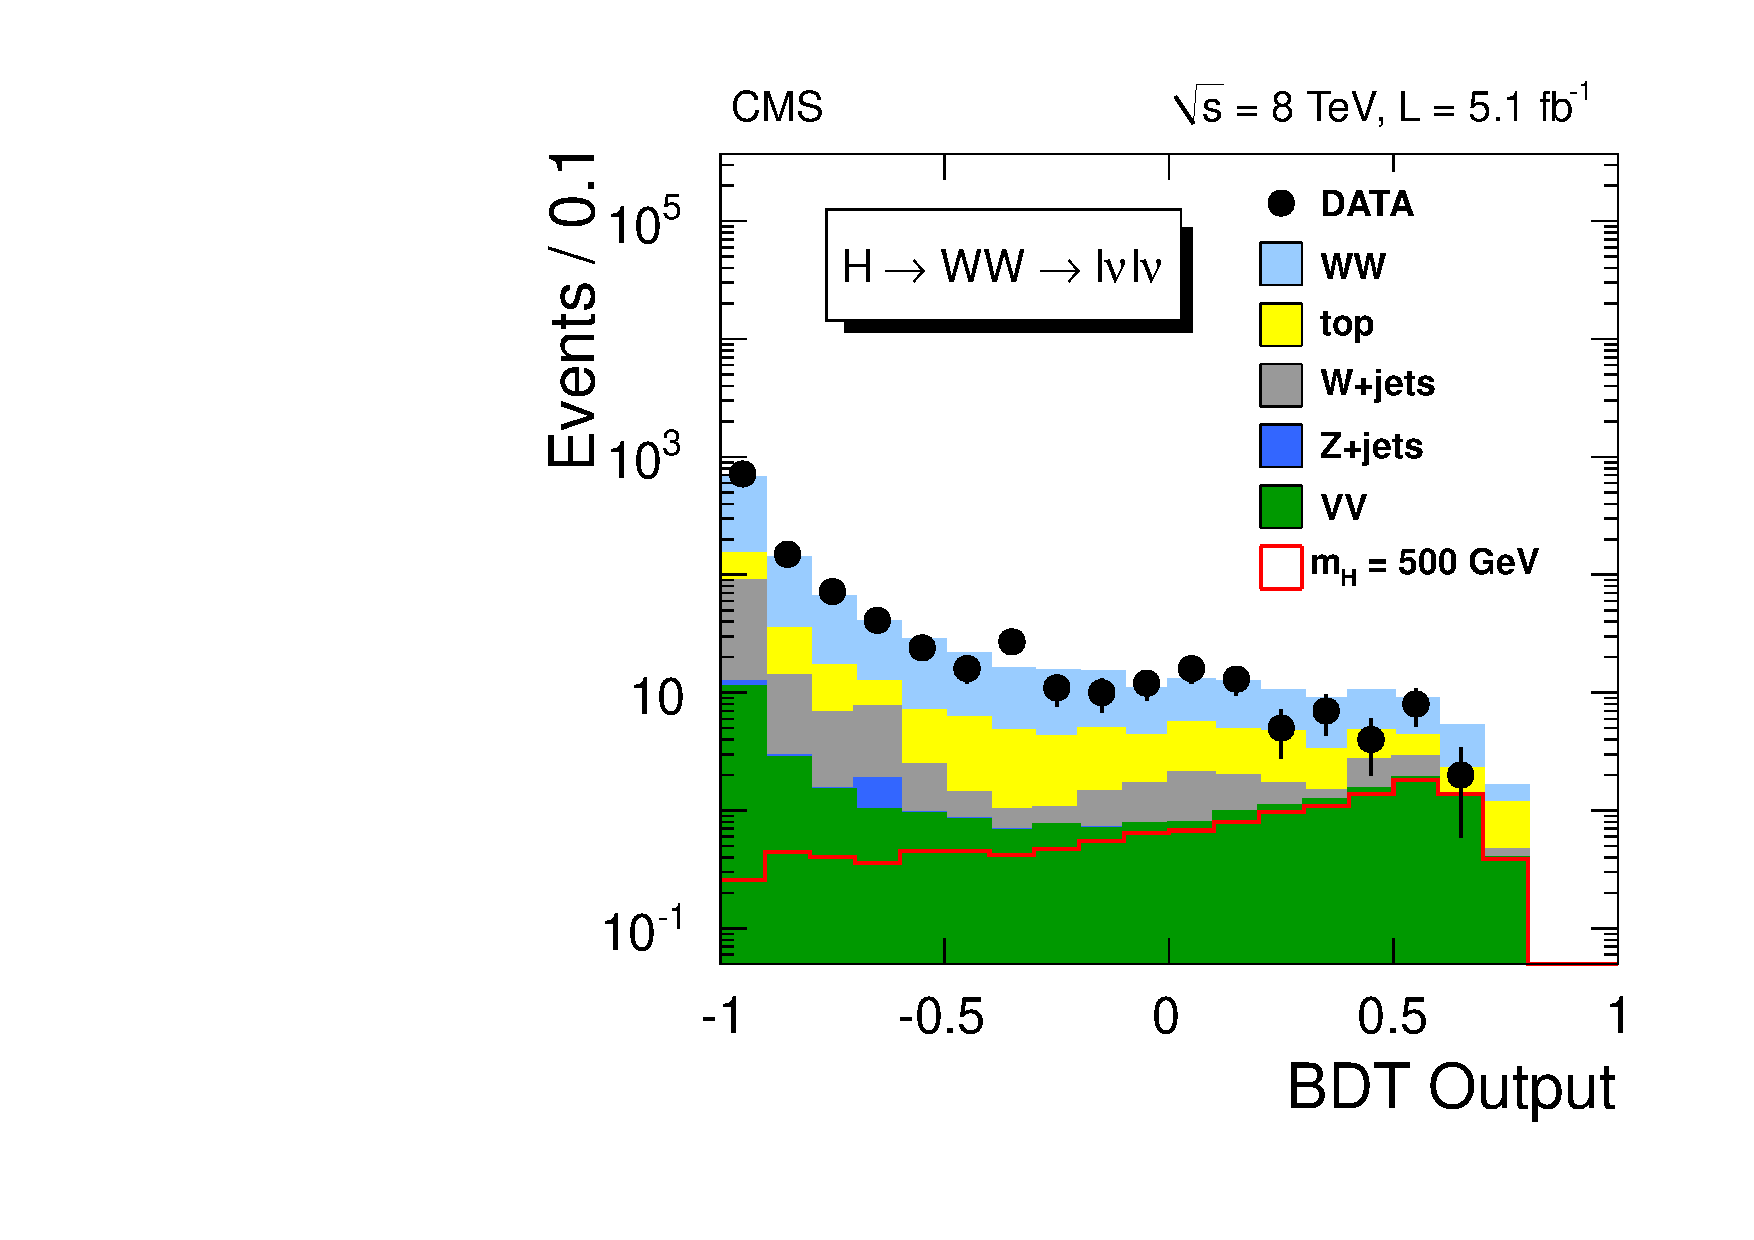
\includegraphics[width=0.49\textwidth]{figures/WW2l2nuBDT.pdf}
   \caption{(a) Distributions of the dilepton mass between the
   two selected leptons in the 0-jet category, for data (points with
   error bars), for the main backgrounds (stacked histograms), and for
   a SM Higgs boson signal with $\mH= 500\GeV$ (superimposed
   histogram). The standard pre-selection is applied.  (b) BDT-classifier
   distributions for signal and background events for a SM
   Higgs boson with $\mH=500\GeV$ and for the main backgrounds at the
   BDT selection level in the 0-jet bin different-flavor final state.}
\label{fig:hww2l2n_bdt_500}
\end{figure}

The backgrounds that remain after applying the final selections are
estimated by a combination of techniques, which are described
in~\cite{cmsobsboson}.  
The $\ttbar$ background is estimated by extrapolation from the observed 
number of events with the b-tagging cut inverted. The Drell-Yan background
measurement is based on extrapolation from the observed number of 
$\Pe^+\Pe^-$, 
$\Pgm^+ \Pgm^-$ events with the $\cPZ$-veto cut inverted. The background 
$\PW$+jets
and QCD multi-jet events is derived from measuring the number of events with
one lepton passing a loose cut on isolation. The probabilities for such 
loosely-isolated fake leptons to pass tight isolation cut are measured in
data 
using multi-jets events. 
The non-resonant $\WW$ contribution is taken from simulation.

%The templates for the BDT are mainly taken from the simulation and
%cross-checked in control samples in data. For the $\Wjets$ background
%the nominal shape is derived from the same data control sample used to
%determine the normalization. The signal efficiency is estimated using
%simulations.

%Residual discrepancies in the lepton reconstruction and identification
%efficiencies between data and simulation are corrected for by
%data-to-simulation scale factors measured using $\dyll$ events in the
%$\Z$ peak region~\cite{CMS:2011aa}, recorded with dedicated unbiased triggers.
%These factors depend on the lepton $\pt$ and $|\eta|$, and
%are typically in the range (0.9-1.0).

Experimental effects, theoretical predictions, and the choice of MC
event generators are considered as sources of uncertainty and
their impact on the signal efficiency is assessed.  The impact on the
kinematic distributions is also considered for the BDT analysis. 
%% The experimental uncertainties on lepton efficiency, momentum scale and
%% resolution, $\MET$ modeling, and jet energy scale are applied to the
%% reconstructed objects in simulated events by smearing and scaling the
%% relevant observables and propagating the effects to the kinematic
%% variables used in the analysis.  Separate $\Pq\Paq\to \WW$ samples are
%% produced with varied renormalization and factorization scales using
%% the \textsc{mc@nlo} generator~\cite{MCatNLO} to address the shape
%% uncertainty in the theoretical model. The kinematic differences with
%% respect to an alternate event generator are used as an additional
%% uncertainty for $\Pq\Paq\to \WW$ (\textsc{madgraph} versus
%% \textsc{mc@nlo}) and top-quark production (\textsc{madgraph} versus
%% \textsc{powheg}).  The normalization and the shape uncertainty on the
%% $\Wjets$ background is included by varying the efficiency for
%% misidentified leptons to pass the tight lepton selection and by
%% comparing to the results of a closure test using simulated samples.
%%
%% The relative uncertainty on the signal efficiency from pile-up is evaluated to be $1\%$.
%% The assigned uncertainty corresponds to shifting the mean of the
%% expected distribution which is used to reweight the simulation
%% up and down by one interaction.
%% The uncertainty assigned to the luminosity measurement is $4.4\%$~\cite{lumiPAS}.
%%
%% The systematic uncertainties due to theoretical ambiguities are separated
%% into two components, which are assumed to be
%% independent. The first component is the uncertainty on the fraction of
%% events categorized into the different jet categories and the effect of jet bin migration.
%% The second component is the uncertainty on
%% the lepton acceptance and the selection efficiency of all other
%% requirements. The effect of variations in parton distribution functions and the
%% value of $\alpha_{s}$, and the effect of higher-order corrections,
%% are considered for both components using the \textsc{pdf4lhc}
%% prescription~\cite{Botje:2011sn,Alekhin:2011sk,Lai:2010vv,Martin:2009iq,Ball:2011mu}.
%% For the jet categorization, the effects of higher-order log terms via
%% the uncertainty in the parton shower model and the underlying event
%% are also considered by comparing different generators. These uncertainties range
%% between 10\% and 30\% depending on the jet category.
%% The uncertainties related to the diboson
%% cross sections are calculated using the \textsc{mcfm} program~\cite{MCFM}.
The overall signal efficiency uncertainty is estimated to be about 20\%
and is dominated by the theoretical uncertainty due to missing QCD
higher-order corrections and PDF uncertainties. The total uncertainty on the background estimations
in the $\Hww$ signal region is about 15\%, which is dominated by the
statistical uncertainty on the observed number of events in the background-control regions.

After applying the final selections, no evidence of
a SM Higgs boson is observed over the mass range. Upper limits 
are derived on the ratio of the product of the Higgs boson 
production cross section and the $\Hi \to \WW$ branching fraction,
$\sigma_{\Hi} \times \mathrm{BR}(\Hi \to \WW)$, and the
SM Higgs expectation, $\sigma/\sigma_\text{SM}$.
%To compute the upper limits the modified frequentist construction
%CL$_{s}$~\cite{Read1,Junk,LHC-HCG} is used. The number of events in
%each bin in the BDT discriminant distribution is modeled as a Poisson
%random variable, whose mean value is the sum of the contributions from
%signal and background processes. All the sources of systematic
%uncertainties are considered.  
The observed and expected
upper limits with all categories combined are shown in
Fig.~\ref{fig:hwwlvlvlim}.
% for the 8~$\TeV$ analysis. The 8~$\TeV$ BDT
%analysis is also combined with the analysis performed at 7~$\TeV$.
%Using the BDT analysis, with the addition of the analysis performed at
%7~$\TeV$, a 
%The Higgs boson with mass in the range 129--560\GeV is
%excluded at 95\% CL, while the expected exclusion limit for the
%background only hypothesis is in the range 122--510\GeV.

\begin{figure}[htbp]
  \centering
%  \subfigure[]{
%  \includegraphics[width=0.48\textwidth]{plots/hwwlvlvlimit8tev.pdf}
%  }  
%   \subfigure[]{ 
  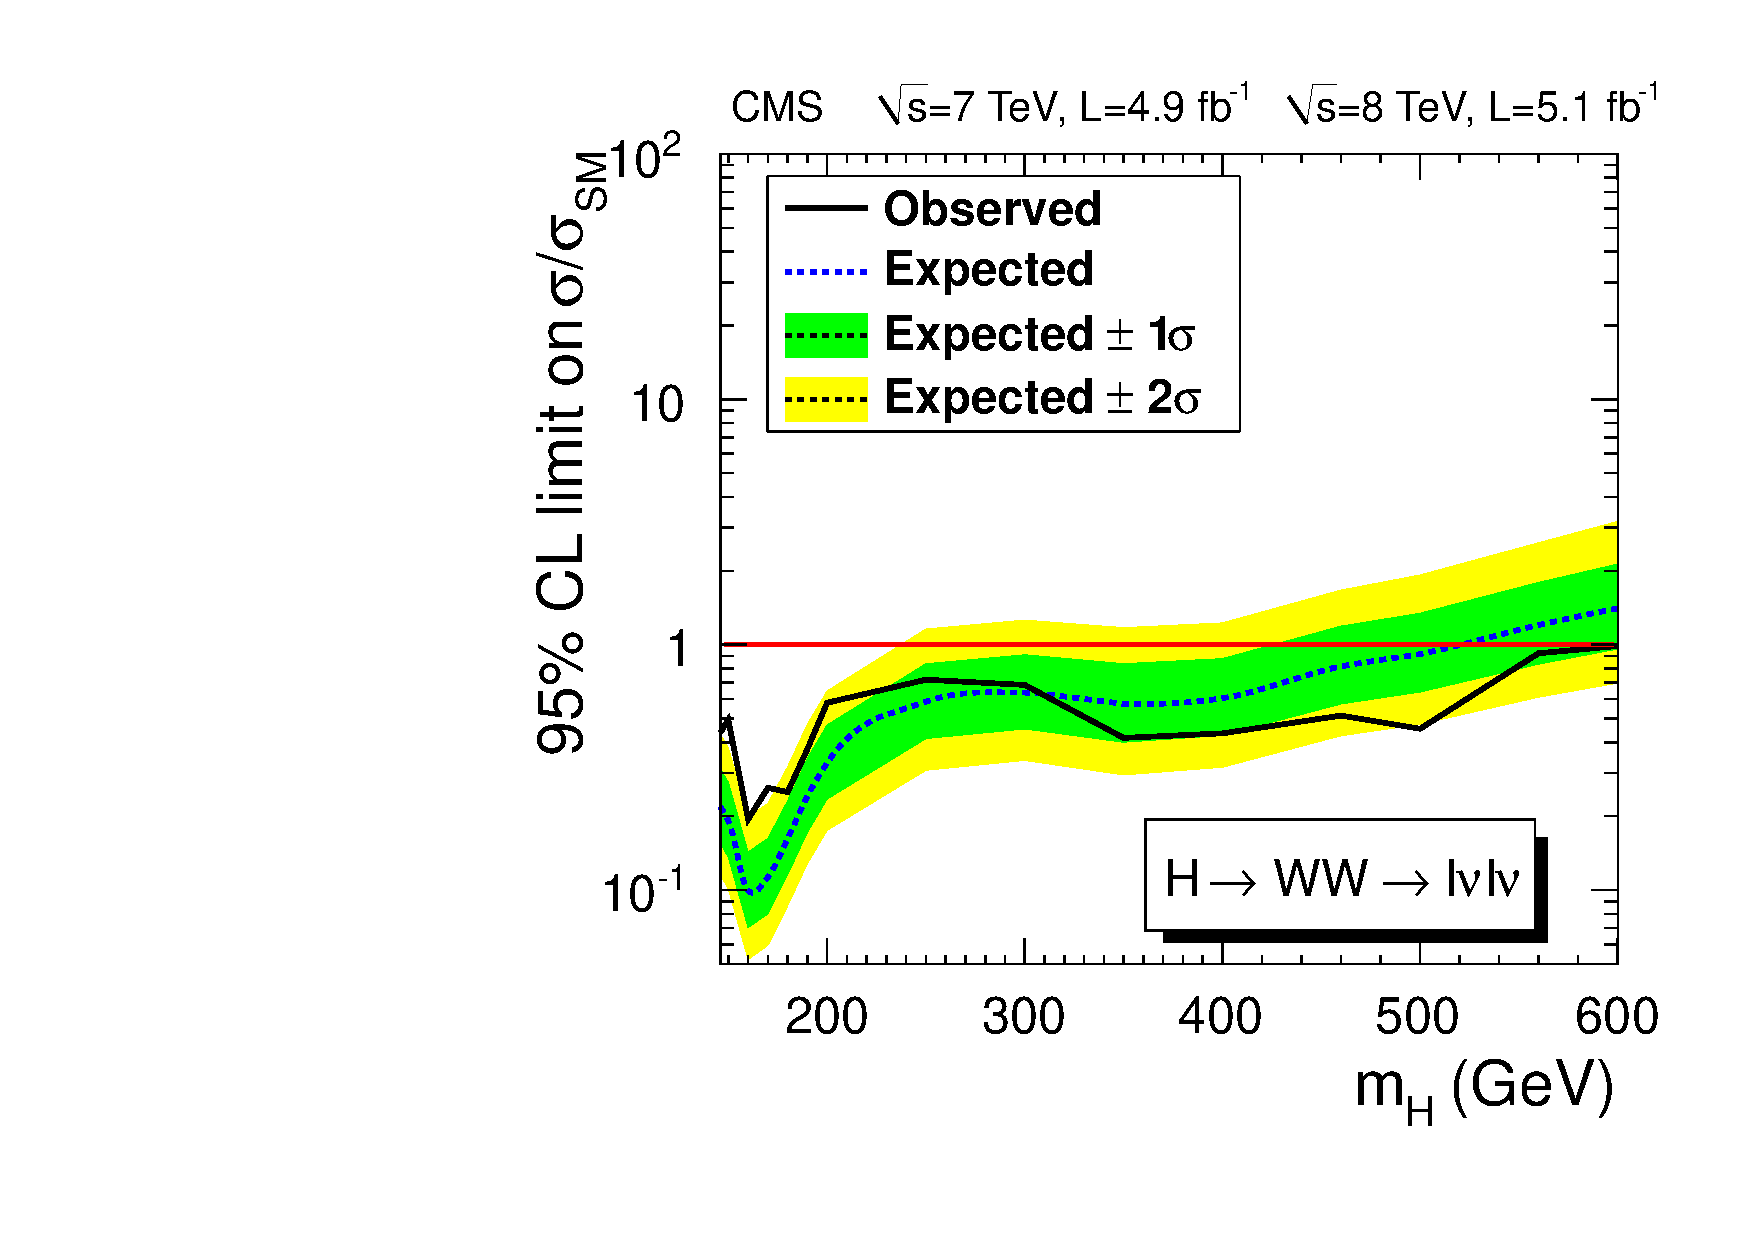
\includegraphics[width=0.6\textwidth]{figures/WW2l2nuLimit.pdf}
%  }   
  \caption{\label{fig:hwwlvlvlim}Observed (solid) and expected
    (dashed) 95\% CL upper limit on the ratio of the production cross
    section to the SM expectation for the Higgs boson obtained using
    the asymptotic CL${}_{\textrm{S}}$ technique. The 68\% and 95\%
    ranges of expectation for the background-only model are also shown
    with green and yellow bands, respectively. The solid line at 1
    indicates the SM expectation.} 
%The limit combines data from both
%    7 TeV and 8 TeV collisions.}
\end{figure}

\subsection{$\PH \to \PW\PW \to \ell\nu \rm{qq}$}

The $\WW$ semileptonic channel has the largest branching fraction of
all the channels presented in this paper. Its advantage over the fully
leptonic final state is that it has a reconstructable Higgs mass
peak~\cite{intro2}. This comes at the expense of a large \PW+jets
background. The level to which this background can be controlled
largely determines the sensitivity of the analysis.

This channel uses data collected with a suite of single lepton
triggers using \pt thresholds 
of 27\GeV for electrons and  
24\GeV
for muons.
Electron triggers are limited to
$|\eta| < 2.5$, while muons are triggered up to $|\eta| < 2.4$.
The reconstructed electrons (muons) are required to have 
%a momentum transverse
%to the beam direction, 
\PT greater than 35(25)\GeV and are
restricted to $|\eta|<$2.5(2.1). 
%Simulated Monte Carlo (MC) samples are corrected for any data-MC
%difference in trigger efficiency.  
%The main sources of background are
%estimated from data.  
%Monte Carlo simulations are used as described
%previously to estimate residual contribution of the background, and to
%estimate efficiency of the Higgs signal.  For this analysis, samples
%with Higgs mass hypotheses ranging from 170 to 600\GeV have been used.

%Objects are reconstructed as described in
%Sec.~\ref{sec:reconstruction}. 
The analysis is performed in four categories with electrons, muons, with
two or three jets
within the tracker acceptance
($|\eta|<2.4$) and with $\PT>30\GeV$.
% are selected for the
%analysis. 
Jets that overlap with isolated leptons are not considered,
where the overlap is determined by a cone around the lepton axis of
radius $\Delta R$ = 0.3. Since initial and final state gluon radiation
can result in an extra jet, only events with two or three jets above
these thresholds within the tracker acceptance are selected for the
analysis.

The combination of the two highest-$\PT$ jets is chosen as the
hadronic $\PW$ candidate.  According to simulation, in the case of 2(3)-jet
events, the correct jet-combination rate varies from 68(26)\% for $\mH = 200\GeV$
to 88(84)\% for $\mH = 600\GeV$.  
%For 3-jet events, the
%corresponding rates are 26\% and 84\%, respectively.  
The events with
the incorrect dijet combination result in a broad non-peaking
background in the $m_{\WW}$ spectrum.

The leptonic $\PW$ candidate is reconstructed from the $(\ell,\MET)$
system. 
%Electrons (muons) are required to have 
%a momentum transverse
%to the beam direction, 
%\PT greater than 35(25)\GeV and are
%restricted to $|\eta|<$2.5(2.1). 
%They are further required to be
%isolated as described in Sec.~\ref{sec:reconstruction}. The $\MET$ is
%measured in the event from the full
%particle-flow~\cite{CMS-PAS-PFT-09-001} reconstruction.  
%The $\MET$ resolution, measured as a function of the sum $\ET$
%($\sum\ET$) of the PF objects in the event, varies from 4\%
%at $\sum\ET=60\GeV$ to 10\% at
%$\sum\ET=350\GeV$~\cite{Chatrchyan:2011tn}.  We require 
The $\MET$ is required to be $\MET>30(25)\GeV$
in the electron (muon) data samples. 
%The transverse
%mass of the leptonic W candidate is defined as {\small $\MT \equiv
%\sqrt{2~p_T^l~\MET~(1-\cos(\phi_l-\phi_{\MET}))}$}, where $\phi_l$ and
%$\phi_{\MET}$ are the azimuthal angles of the lepton and $\MET$,
%respectively.  
To reduce the background from processes that do not
contain $\PW\to\ell\nu$ decays, we require $m_{\rm{T}}^{\ell,\MET}>30\GeV$,
and,
to reduce the QCD multi-jet background,
$|\Delta\phi_{\textrm{leading jet,MET}}| >$ 0.8 (0.4) for
electrons (muons).

To improve the $m_{\WW}$ resolution, both $\PW$ candidates are constrained
in a kinematic fit to the $\PW$-boson invariant mass to within its known
width, with the unmeasurable longitudinal component of the neutrino
momentum, $|p_{\textnormal{z}}|$, being the unknown.The ambiguity in
the second-order equation is resolved by taking the solution that
yields the smallest $|p_{\textnormal{z}}|$ value for the neutrino.  

To exploit the differences in kinematics between signal and
background, a likelihood discriminant is constructed that incorporates
a set of variables that best distinguishes the Higgs signal from the
\PW+jets background. 
%This approach improves the expected sensitivity to
%a Higgs mass hypothesis across the entire mass range. 
These variables
comprise five angles between the Higgs decay products that fully
describe the Higgs production kinematics~\cite{Gao:2010qx}, the $\PT$
and rapidity of the $\WW$ system, and the lepton charge.
The likelihood discriminant is optimized with dedicated simulation
samples for several discrete Higgs-mass hypotheses, for each lepton
flavor ($\Pe$, $\Pgm$) and for each jet multiplicity (2 jets, 3 jets)
independently.  In this way, four different optimizations are obtained
per mass hypothesis.  For each of them, events are retained if they
survive a simple selection on the likelihood discriminant, chosen on
the basis of the expected limit for the Higgs extraction as the figure
of merit.

%The remainder of the analysis in this channel consists of a two-body
%fit of the invariant mass $m_{jj}$ of the dijet system, which is the
%hadronic W candidate, and a construction of the shape of the four-body
%of invariant mass $m_\textnormal{WW}$ distribution of the $\ell\nu jj$
%system, which is the combined WW system.

To extract simultaneously the relative normalizations of all
background components in the signal region, an unbinned maximum
likelihood fit is performed on the invariant mass of the dijet system,
$m_{jj}$.  The fit is done for each Higgs mass hypotheses
independently.  The signal region corresponding to the $\PW$ mass window,
$65\GeV < m_{jj} < 95\GeV$, is excluded from the fit.  The shape of the $m_{jj}$ 
distribution for the $\PW$+jets background
is taken from simulation for Higgs mass hypotheses at or below
200\GeV. For higher masses the simulation doesn't have enough events,
so we describe the shape analytically using an exponential fit
function.  The overall normalization of the \PW+jets component is
allowed to vary in the fit.  The shapes for othe backgrounds,
electroweak diboson, \ttbar, single
top, and Drell-Yan+jets are based on simulation and their
normalization are constrained to the theoretical predictions, within
the corresponding uncertainties.
The multijet-background normalization is derived from data by relaxing
lepton isolation and identification requirements. Its contribution to
the total number of events is evaluated from a separate two-component
likelihood fit to the $m_{\rm{T}}^{\ell,\MET}$ distribution, and constrained
in the $m_{jj}$ fit according to this fraction within
uncertainties. 
For electrons the multijet fraction accounts for several percents depending on the number 
of jets
in the event, while for
muons it is negligible.

The limits are set based on the measured invariant mass of the $\WW$
system, 
$m_{\ell\nu jj}$.  The binned shapes of $m_{\ell\nu jj}$ for total
background, signal and data for each mass hypothesis and event
category are constructed.
%, and these shapes are fed to the limit
%setter.  
The $m_{\ell\nu jj}$ shape for the major background,  
\PW+jets,
is
extracted from data as a linear combination of the shapes measured in
two signal-free sideband regions of $m_{jj}$, namely an upper sideband
($95\GeV <m_{jj} < 115\GeV$ ) and a lower sideband ($55\GeV <m_{jj} <
65\GeV$).  The relative fraction of the two sidebands is chosen from
simulation, separately for each Higgs mass hypotheses, by
minimizing the $\chi^2$ between the extrapolated shape in the signal
region and the expected one.

The $m_{\ell\nu jj}$ shape for multijet background events is obtained
from data sample selected for the
$m_{jj}$ fit and normalized according to the fit results.
All other background categories use the $m_{\ell\nu{}jj}$ shape
from simulation.

Examples of the $m_{jj}$ and $m_{\ell\nu jj}$ fits are shown in
Fig.~\ref{fig:lvjjfits}, with selections optimized for Higgs mass
hypothesis 500\GeV, for $(\Pgm,2\rm{jets})$ category.  The distributions of
the extrapolated \PW+jets background in the signal region are also
shown.  Because of the low statistics, the shapes are regularized by
means of an exponential fit (solid curve). The uncertainties from both
fits are propagated to the limit calculation as systematic
uncertainties.

\begin{figure}[htbp]
  \centering
  \subfigure[]{
%  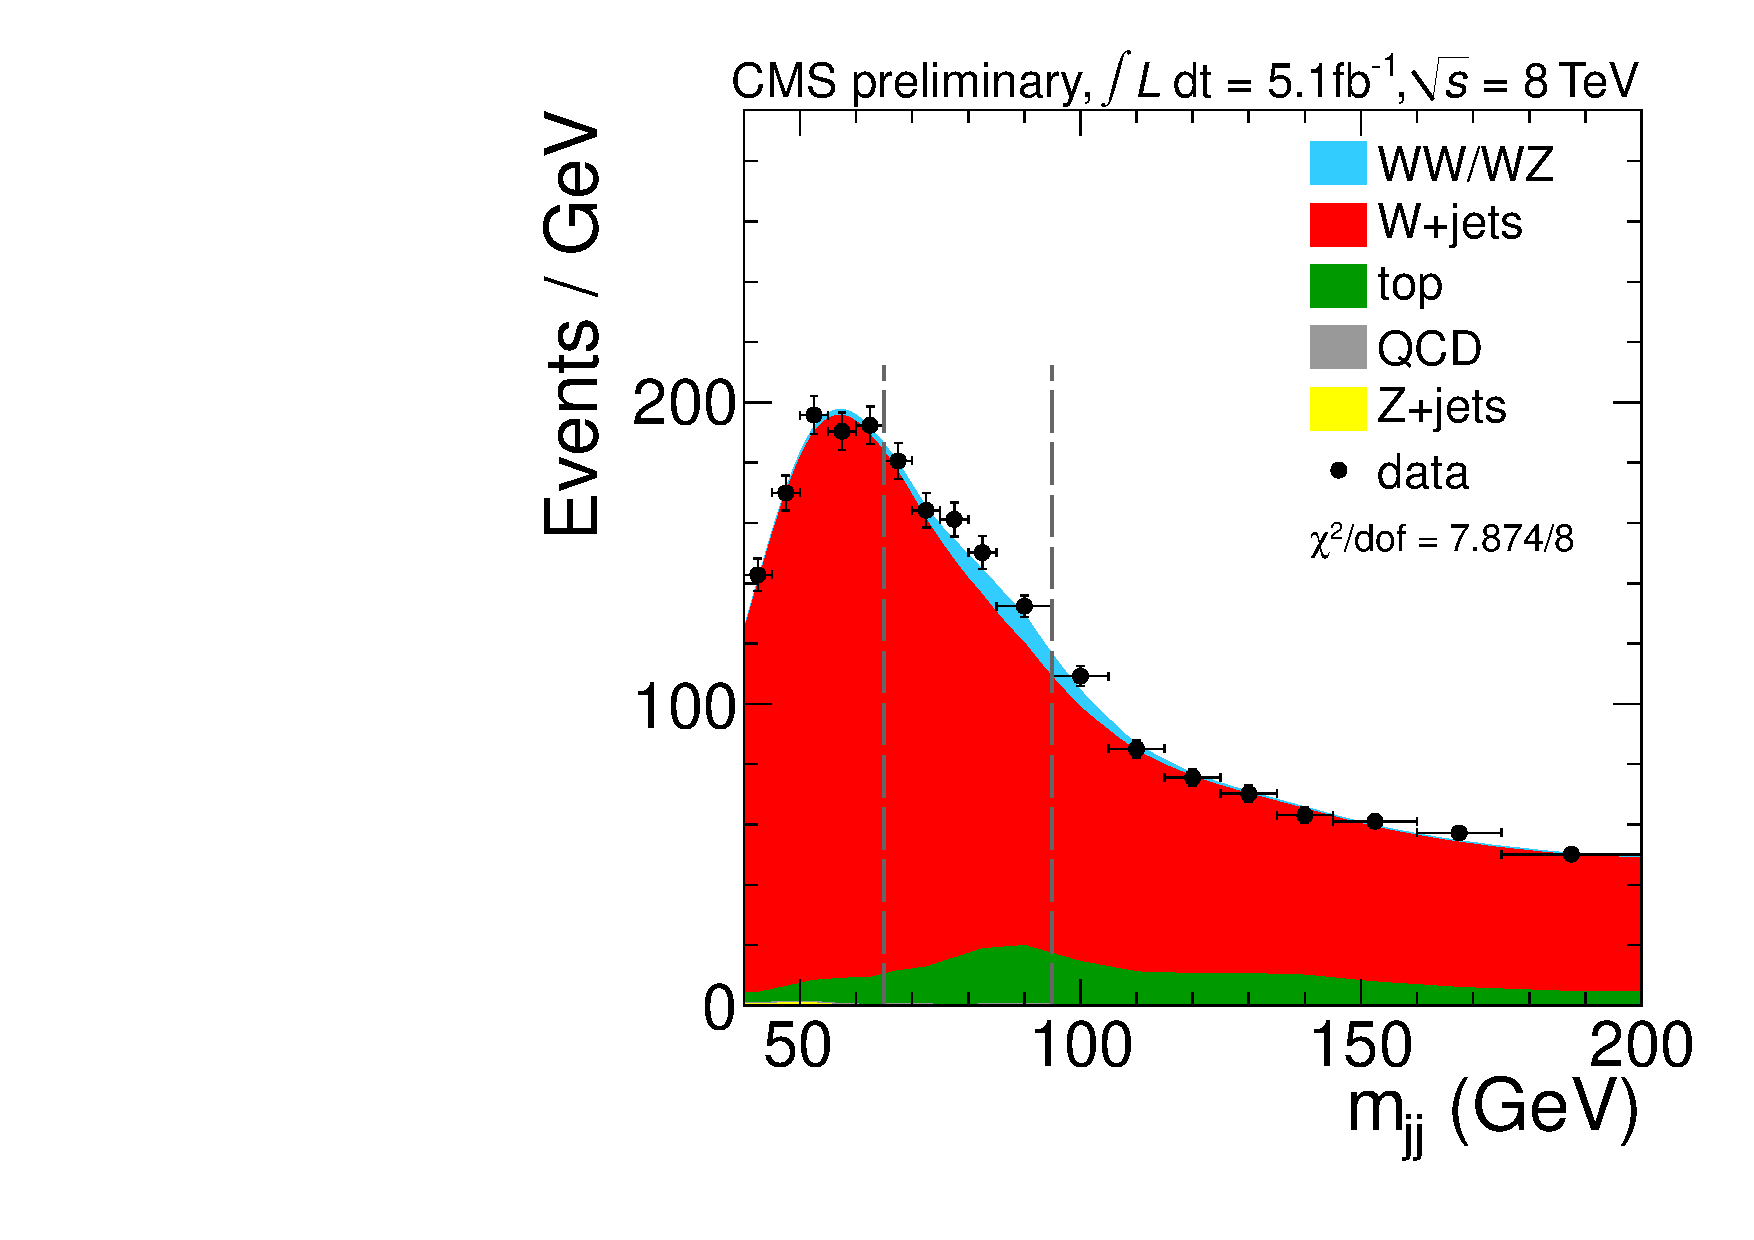
\includegraphics[width=0.48\textwidth]{plots/H500_Mjj_Muon_2jets_Stacked.pdf}
  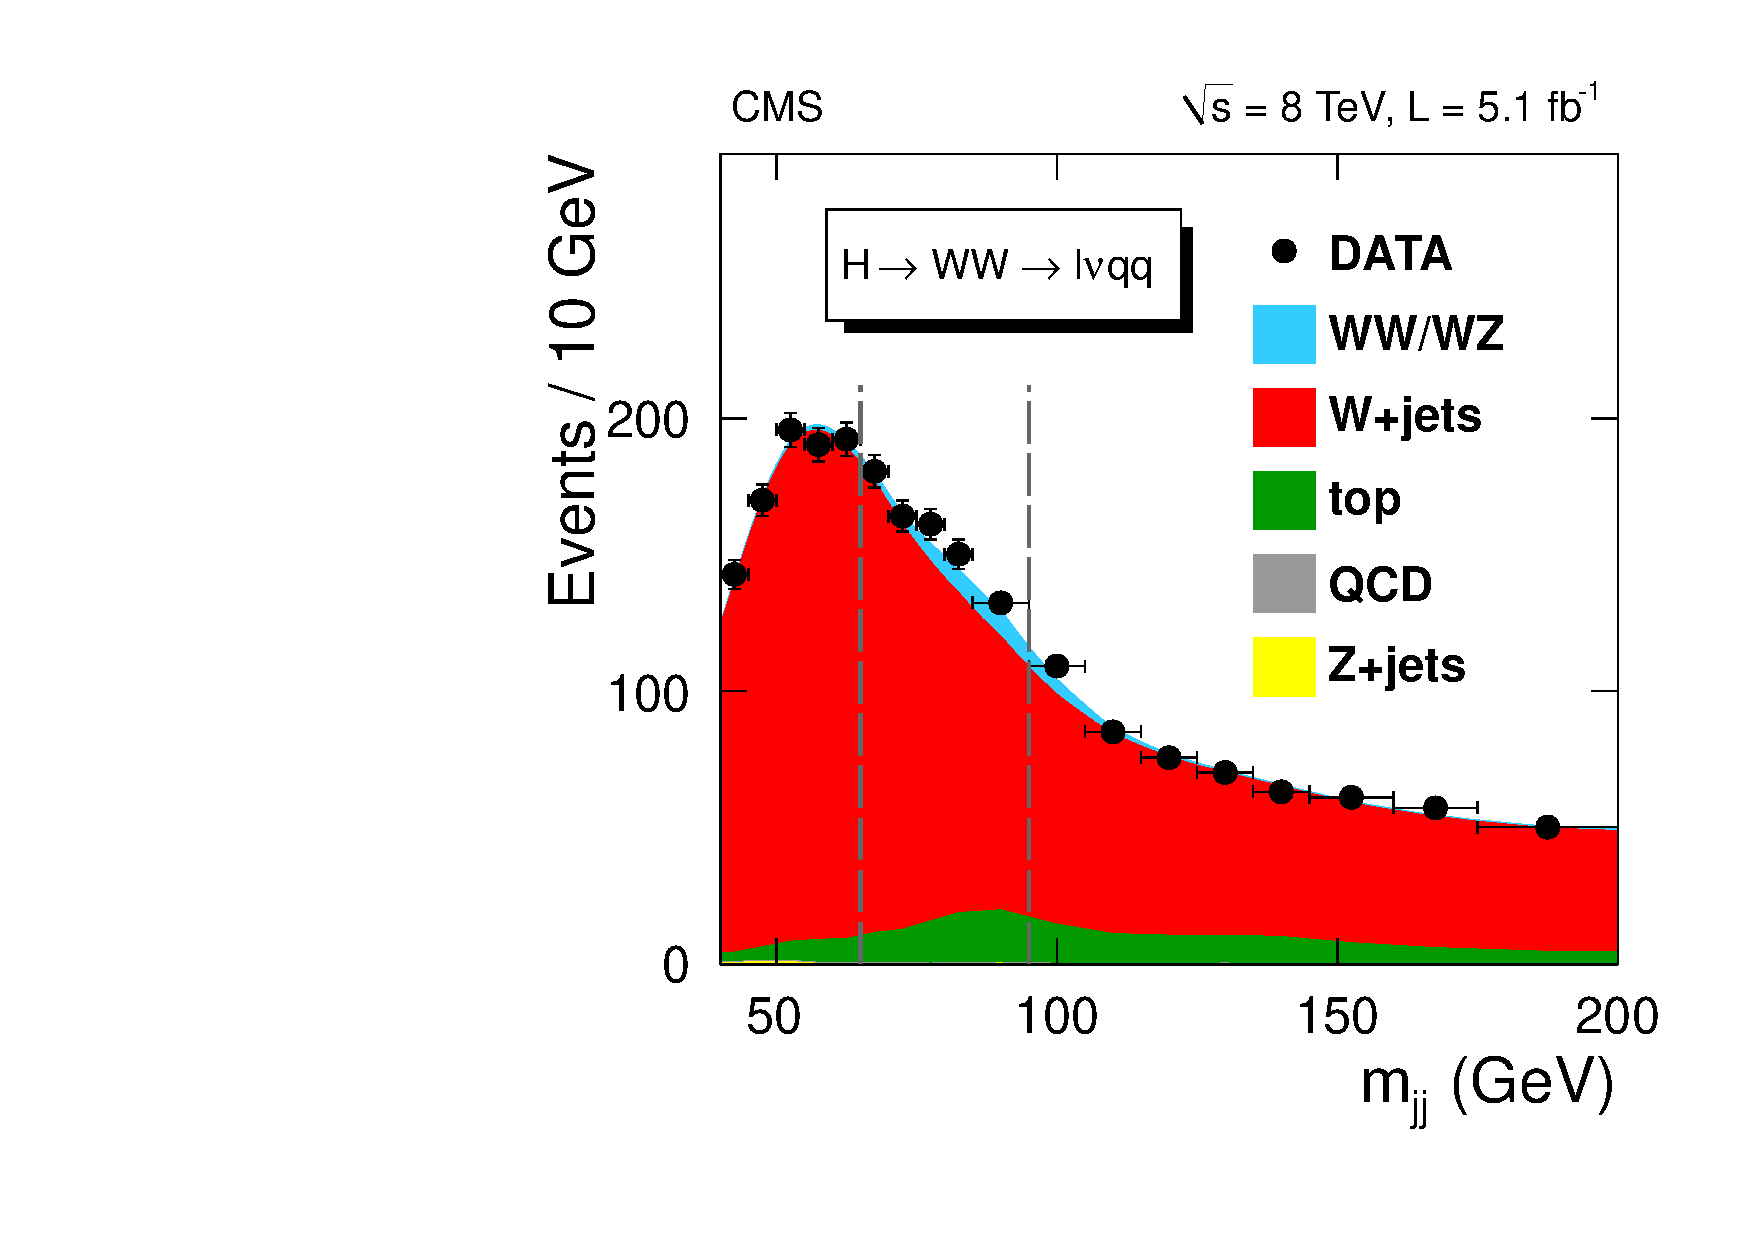
\includegraphics[width=0.48\textwidth]{figures/WW2l2qMjj.pdf}
  }  
   \subfigure[]{ 
%  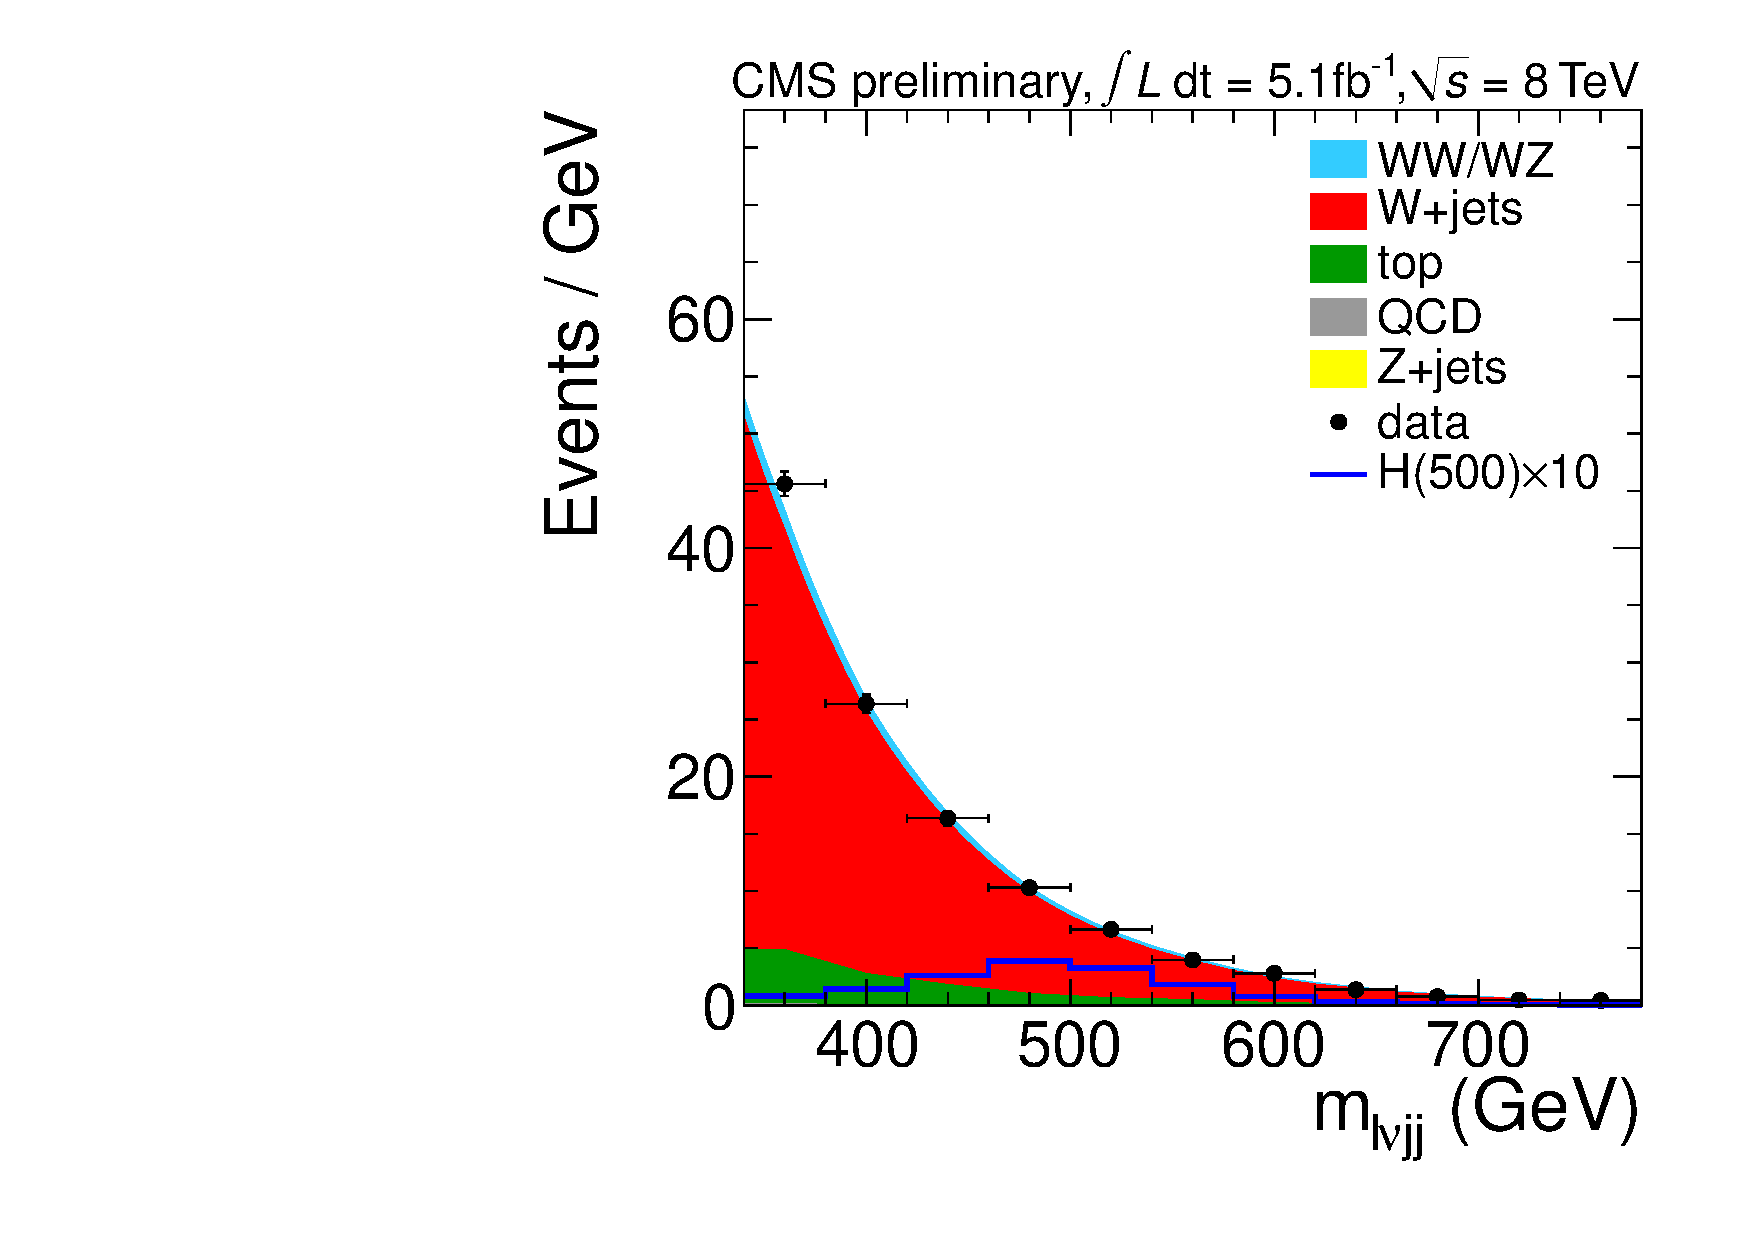
\includegraphics[width=0.48\textwidth]{plots/H500_Mlvjj_Muon_2jets_Stacked.pdf}
  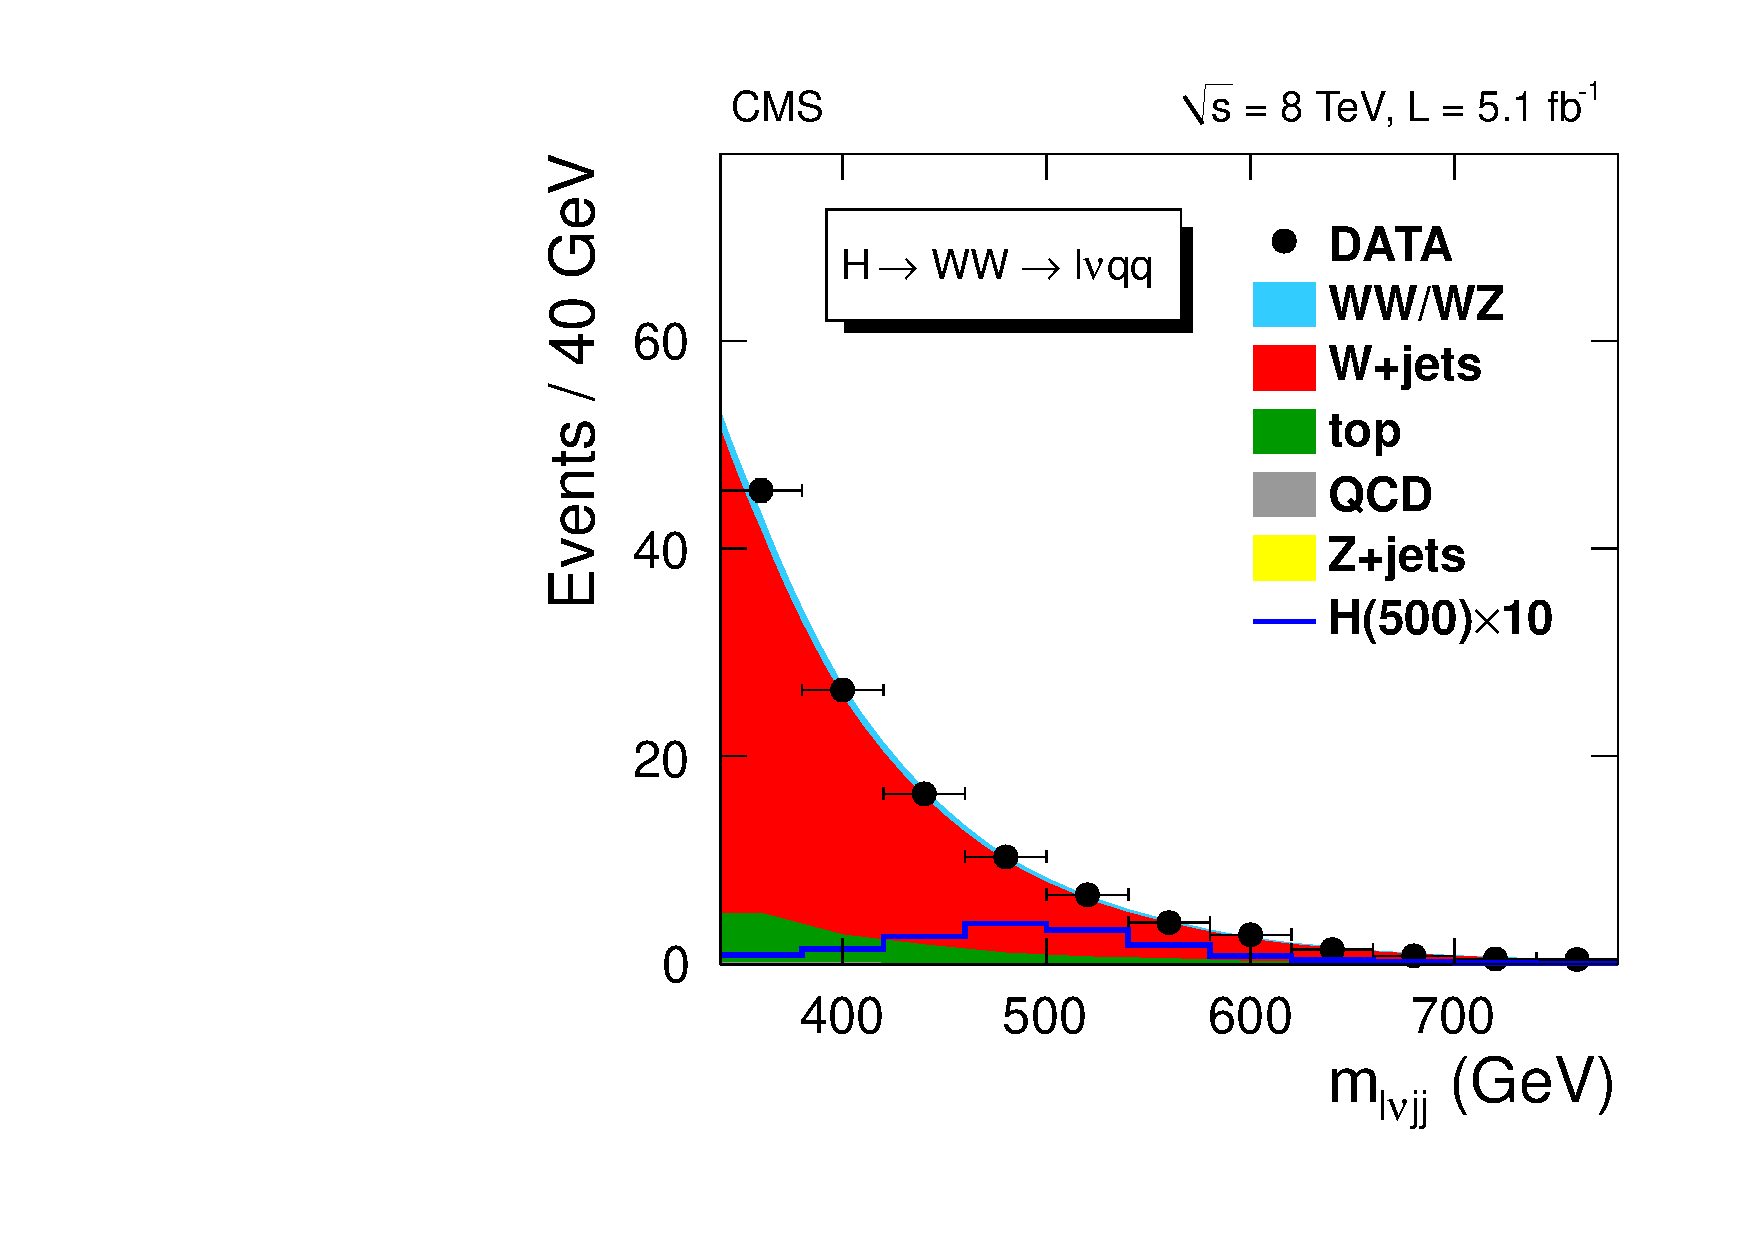
\includegraphics[width=0.48\textwidth]{figures/WW2l2qMass.pdf}
  }   
%  \subfigure[]{ 
%  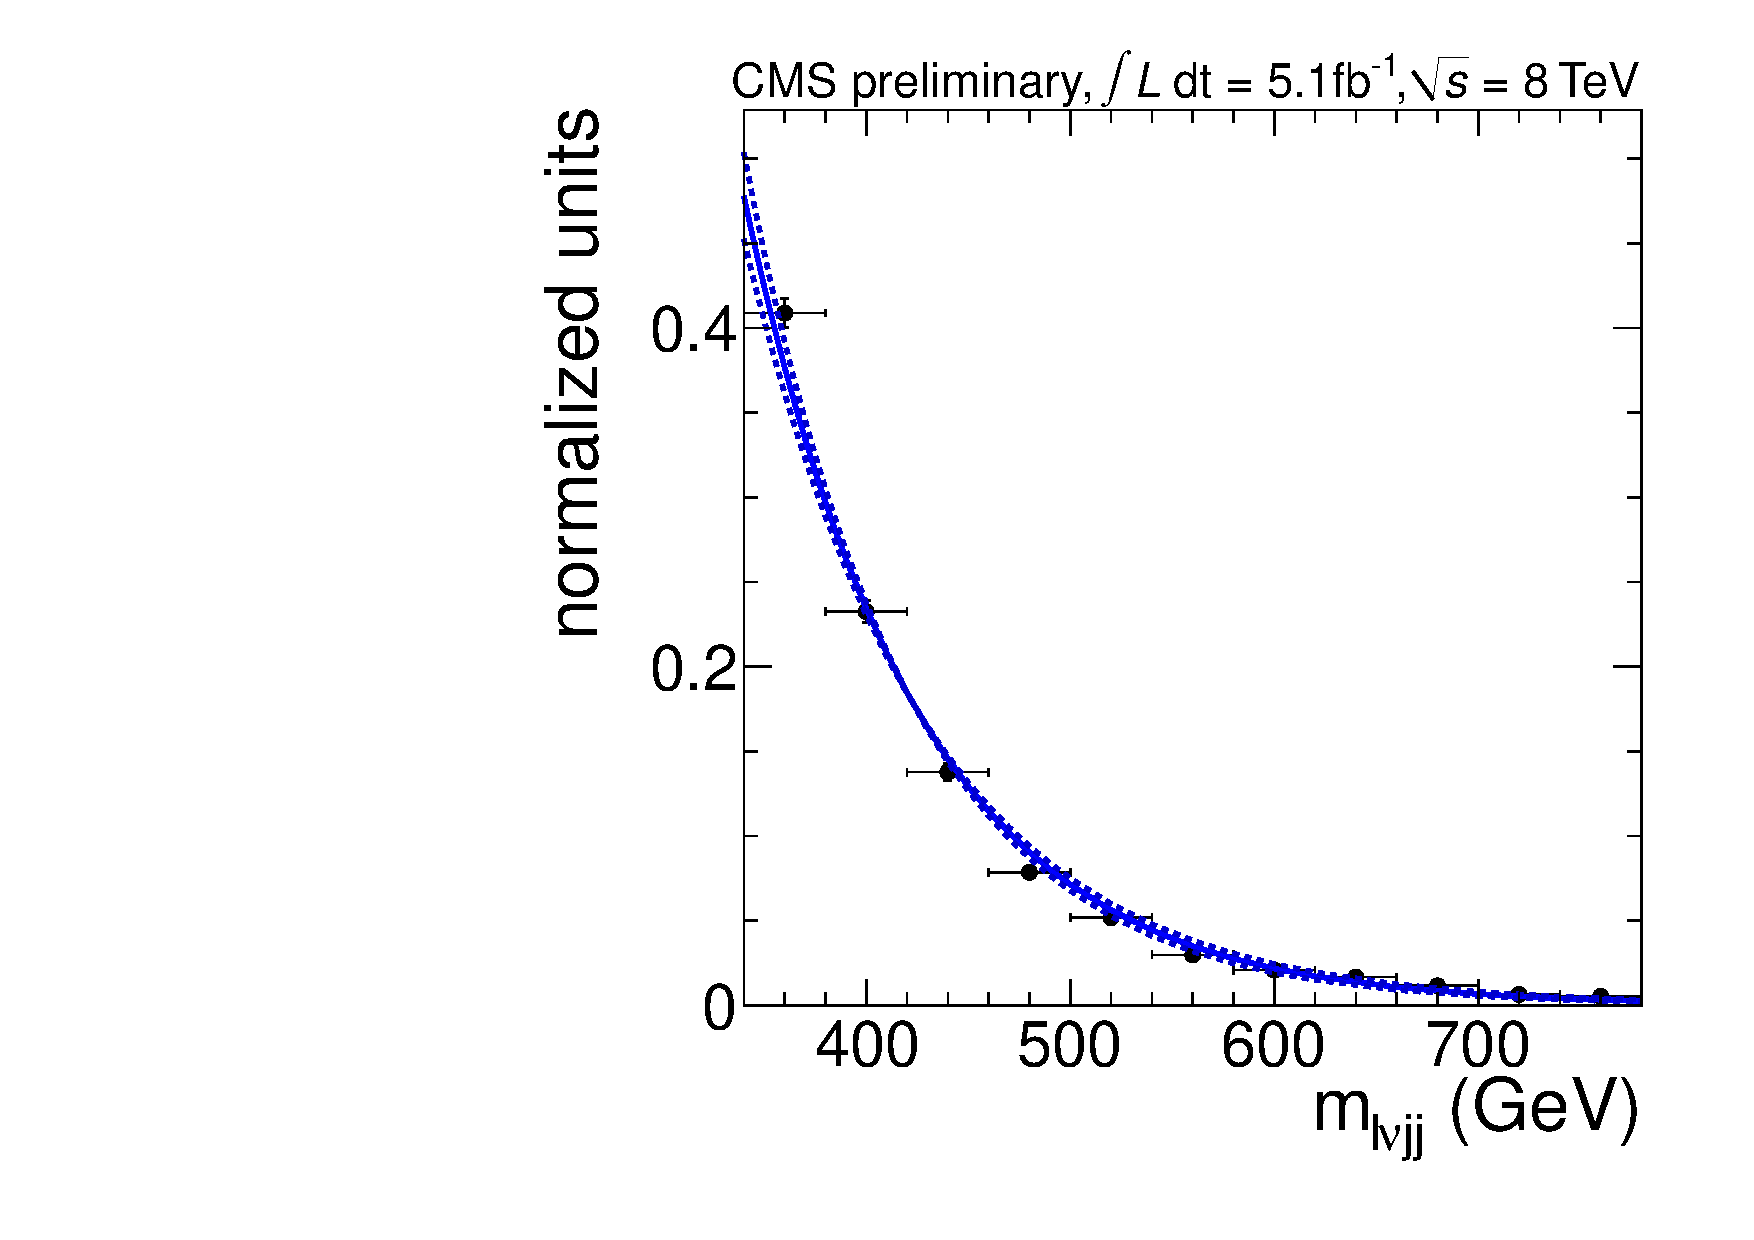
\includegraphics[width=0.32\textwidth]{plots/H500_Mlvjj_Muon_2jets_WpJShape.pdf}
%  }  
  \caption{\label{fig:lvjjfits} Fit plots for the mass hypothesis
    $\mH=500\GeV$, muon 2-jet category.  (a) The dijet invariant mass
    distribution with the fit projections of the background components.
    The vertical lines corresponds to the signal region of this analysis
    $65\GeV < m_{jj}
    < 95\GeV$.  %(c) The distribution of the extrapolated background
    (b) The \WW invariant mass distribution with the fit projections of
    the background components in the signal region.
    %(c) The distribution of the extrapolated background
%    shape in the signal region.  
    The black markers represent the
    extrapolated points, while the blue curve is the smooth
    parametrization using an exponential function.  The dashed bands
    show the envelope of the systematic uncertainty in the shape
    extrapolation. }
\end{figure}

%Because of the background dominance, 
The largest source of systematic
uncertainty is due to $m_{\ell\nu jj}$-shape uncertainty of the \PW+jets background.
% $m_{\ell\nu jj}$
%distribution.
% described in the previous section.  
The only other
uncertainty assigned to background is the normalization uncertainty
from the $m_{jj}$ fit. Both of these uncertainties are
estimated from data. All other systematic uncertainties are applied to
signal processes. The dominant signal uncertainties include
theoretical uncertainties for the cross section (14-19\% for gluon
fusion)~\cite{LHCHiggsCrossSectionWorkingGroup:2011ti} and exclusive
jet binning effects on scale (4-28\%), as well as the efficiency of
the likelihood selection (10\%). The latter effect is computed by
taking the relative difference in efficiency between data and
simulation using a control sample of top pair events in data. These
events are good proxies for our signal because in both cases the
primary production mechanism is gluon-gluon fusion and the
semi-leptonic final state contains decays of two W bosons.

%We observe no evidence for the SM Higgs boson and
%. We therefore 
%present
The upper limits on the ratio of the production cross section for the
Higgs boson compared to the SM expectation are presented in
Fig.~\ref{fig:hwwlvjjlim}. 
%When combined with 5.1\fbinv
%of 7 TeV data collected in 2011, we 
%We exclude the SM Higgs boson in the
%mass range 230--480~\GeV, at 95\% confidence level.

\begin{figure}[htbp]
  \centering
%   \subfigure[]{
%  \includegraphics[width=0.48\textwidth]{plots/hwwlvjjlimit8tev.pdf}
%   }
%  \subfigure[]{
  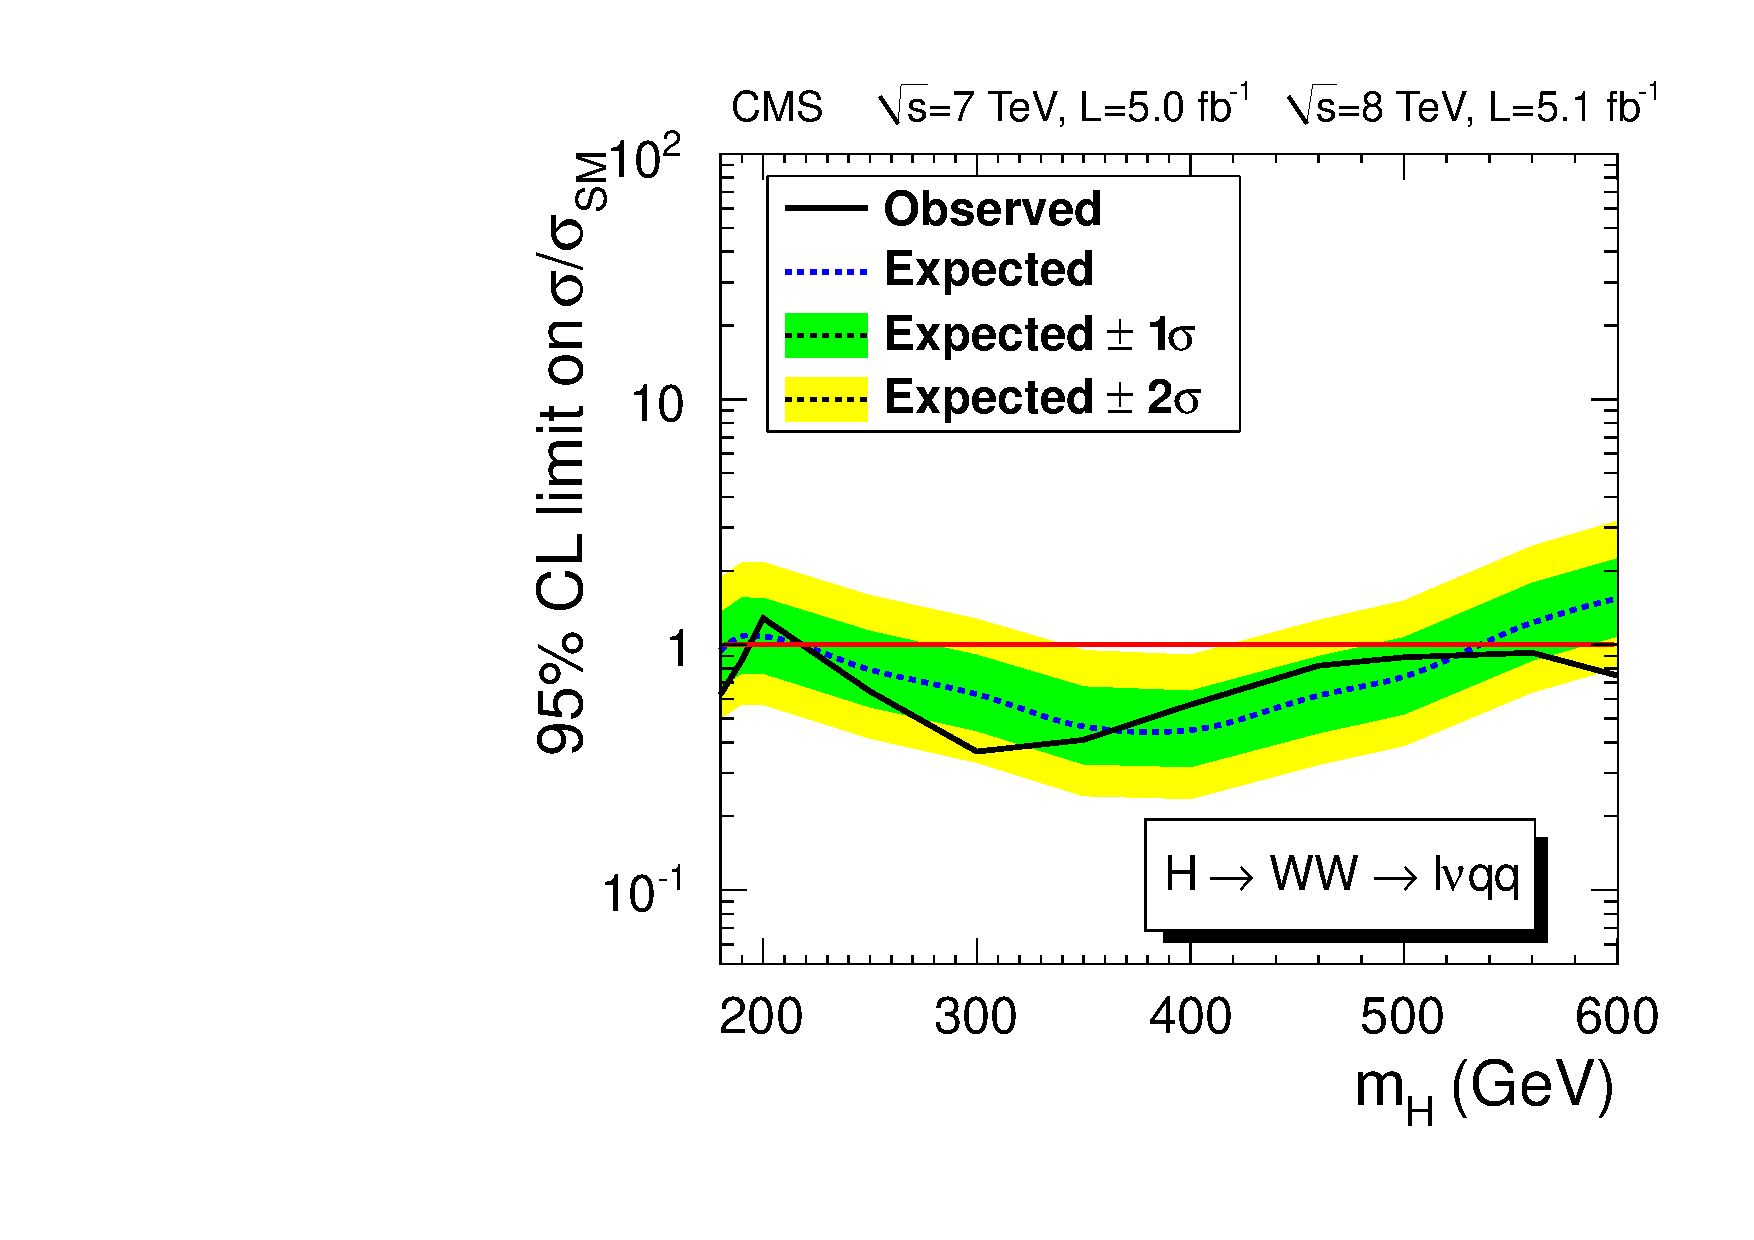
\includegraphics[width=0.6\textwidth]{figures/WW2l2qLimit.pdf}
%  }
  \caption{\label{fig:hwwlvjjlim}Observed (solid) and expected
  (dashed) 95\% CL upper limit on the ratio of the production cross
  section to the SM expectation for the Higgs boson in the WW
  semileptonic channel.}  
%The limit combines data from both 7 TeV and 8
%  TeV collisions.}
\end{figure}
